\section { Parameterization of the Detector Response}

As published RMC spectra have the detector response convoluted in, to compare
them to the model predictions one needs to know the detector response.

Fortunately, the TRIUMF group which has published the most recent highest statistics
RMC spectra, has also made published its detector response -
see \cite{RMC_1992_PhysRevC.46.1094} and \cite{RMC_1998_PhysRevC.58.1767}. 

The detector response D(E,E') is defined as the probability for a photon
with energy E to be reconstructed in the detector with energy E'. As follows from the
definition, D(E,E') includes both resolution and acceptance - the integral of D(E,E')dE'
gives the total acceptance for a given energy E.

In both \cite{RMC_1992_PhysRevC.46.1094} and \cite{RMC_1998_PhysRevC.58.1767}, the
detector response is determined using the GEANT3-based simulation using monoenergetic
photons in a energy range of 50-140 MeV, and parameterized analytically.
The parameterizations of  \cite{RMC_1992_PhysRevC.46.1094} and \cite{RMC_1998_PhysRevC.58.1767}
are significantly different, the source of the difference is not understood.

%%%%%%%%%%%%%%%%%%%%%%%%%%%%%%%%%%%%%%%%%%%%%%%%%%%%%%%%%%%%%%%%%%%%%%%%%%%%%%
\subsection { 1992 Detector response parametrization (\cite{RMC_1992_PhysRevC.46.1094})}

The response of the TRIUMF RMC spectrometer published in \cite{RMC_1992_PhysRevC.46.1094}
is described as a Gaussian function with the exponential low- and  high-energy tails.
In order to reproduce the low-energy resolution tail for high-energy photons, a second Gaussian
is added for the photon energy E>60 MeV. The functional form is as follows:

\begin{equation}
  \label{eq:001}
\text{D(E,E')}= \left\{
\begin{array}{ll}
                \text{A exp}\left[-\frac{1}{2\sigma_0^2}(E'-E_o)\right]+
                \text{F exp}\left[-\frac{1}{2\sigma_3^2}(E'-E_3)^2\right]
 \quad E_1<E'<E_2 \\
                \text{B exp}\left[-\frac{1}{\sigma_1}(E_1-E') \right]+
                \text{F exp}\left[-\frac{1}{2\sigma_3^2}(E'-E_3)^2\right]
 \quad E'<E_1      \\  
                \text{C exp}\left[-\frac{1}{\sigma_2}(E'-E_2)\right]+
                \text{F exp}\left[-\frac{1}{2\sigma_3^2}(E'-E_3)^2\right]
 \quad E'>E2     
 \end{array}
 \right\}
\end{equation}
 
where $E_1=E_0 - \frac{\sigma_0^2}{\sigma_1}$, $E_2 =E_0 + \frac{\sigma_0^2}{\sigma_2}$,
 $B=\text{A exp}\left[-\frac{\sigma_0^2}{2\sigma_1^2}\right]$, 
 $C=\text{A exp}\left[\frac{\sigma_0^2}{2\sigma_2^2}\right]$. 

 The parameters $A, B ,C , F, \sigma_i$  etc are polynomials in the photon energy:
 
\begin{equation}
  f(E)= P_0+P_1E+P_2E^2+P_3E^3
\end{equation}

The coefficients are reported in tables ~\ref{tab:coefficients1} and ~\ref{tab:coefficients2} .

\begin{table}[!h]
\begin{center}
\begin{tabular}{| c | c | c | c | c | }
\hline
Parameter & $P_0$ (MeV)& $P_1$ & $P_2$ (MeV)$^{-1}$ \\ \hline
$\sigma_0$ & -0.5836 & 0.0352 & \\ \hline
$\sigma_1$ & -5.879 & 0.1653 & -5.149$\times 10^{-4}$ \\ \hline
$\sigma_2$ & 1.596 & -0.03859 & 3.883$\times 10^{-4}$ \\ \hline
$\sigma_3$ & -47.80 & 1.010 & -4.406$\times 10^{-3}$ \\ \hline
E$_3$ & 1.068 & 0.7507 & \\ \hline
E$_0$ (E>60) & -1.161 & 0.9481 & 1.724$\times 10^{-3}$ \\ \hline
E$_0$ (E<60) & 22.73 & 0.1995 & 5.993$\times 10^{-3}$ \\ \hline

\end{tabular}
\end{center}
\caption{
  Polynomial parameterization of the coefficiencts in \ref{eq:001}
  \label{tab:coefficients1}}
\end{table}

\begin{table}[!h]
\begin{center}
\begin{tabular}{| c | c | c | c | c | c |}
\hline
Parameter & $P_0$ & $P_1$ (MeV)$^{-1}$ & $P_2$ (MeV)$^{-2}$  & $P_3$ (MeV)$^{-3}$\\ \hline
A & 3.259$\times 10^{-4}$ & -4.120$\times 10^{-4}$ & 1.015$\times 10^{-5}$ & -4.05$\times 10^{-8}$  \\ \hline
F/A & -0.1337 & 2.828$\times 10^{-3}$ & -9.701$\times 10^{-6}$ & \\ \hline
\end{tabular}
\end{center}
\caption{Polynomial parameterization of coefficients in \label{tab:coefficients2}}
\end{table}

In Fig.~\ref{fig:parameterDependance} the photon energy dependence of the parameters of the detector response function are plotted.
\begin{figure}[!h]
 \begin{center}
 \includegraphics[width=0.33\columnwidth]{png/sigmas92.png} 
 \includegraphics[width=0.33\columnwidth]{png/A_FoverA92.png} 
 \includegraphics[width=0.33\columnwidth]{png/E092.png} 
 \end{center}
 \caption{
   Energy dependence of parameters defining the TRIUMF RMC spectrometer response
   \cite{RMC_1992_PhysRevC.46.1094}
 }
 \label{fig:parameterDependance}
 \end{figure}

Some examples of the detector response at different energies, namely 50 MeV , 70 MeV , 90 MeV, and 110 MeV,
 are reported in Fig.~\ref{fig:92ResponseExample}.\\
As previously described, for photon energies E>60 MeV, the low-energy tails are well evident.

\begin{figure}[!h]
\centering
\includegraphics[width =\textwidth]{png/Resp_example92.png}
\caption{'1992 detector response parametrization for different photon energies}
\label{fig:92ResponseExample}
\end{figure}


\subsection { 1998 Detector Response }

The TRIUMF RMC spectrometer response published in 1998 (\cite{RMC_1998_PhysRevC.58.1767}) is
significantly different from its '1992 version.
It s parameterized as a gaussian with logaritmic low-energy and an exponential
high-energy tails:

\begin{equation}
  D(E,E')= \left\{
    \begin{array}{ll}
      \gamma ln(x)/x          \qquad E' \leq (E_0-\sigma_0) \\
      Ae^{-(E'-E_0)^2/2\sigma_0^2} \qquad E0-\sigma_0<E'<(E_0-\sigma_0^2/\sigma^2) \\
      Ae^{-(E'-E_0)/2\sigma_2}    \qquad E' \geq (E_0+\sigma_0^2/\sigma_2)
    \end{array}
  \right\}
\end{equation}

The parameter $\beta$  allows the matching of the low-side and core of the distribution at E'=$E_0-\sigma_0$.

The quantity $x$ is defined as: 
$$x= \frac{\alpha- E}{\alpha -37 \text{ MeV}}$$.
Also in this case the parameters $\alpha,A,E_0,\sigma_0,\sigma_2$ have a polynomial dependence on the photon energy that can be parametrized as:

\begin{equation}
\alpha= a+0+a_1y+a_2y^2+a_3y^3
\end{equation}

where $y= (E-60 \text{MeV}/60 \text{ MeV})$/


The  coefficient of the parameters are reported in Tab.~\ref{tab:param98}
\begin{table}[!h]
\begin{center}
\begin{tabular}{| c | c | c | c | c | c | }
\hline
Parameter & $a_0$ & $a_1$ & $a_2$ & $a_3$ \\ \hline
$\alpha$ & 56.1 &62.5 & -0.826 & 0.0  \\ \hline
A & 9.41$\times 10^{-4}$ & 2.61$\times 10^{-3}$ &0.27 $\times 10^{-2}$ &0.835$\times 10^{-3}$   \\ \hline
$E_0$ & 54.4 & 57.7 & -0.315 &0.0 \\ \hline
$\sigma_0$ & 2.03 &10.4 &1.25 & -0.428\\ \hline
$\sigma_2$ & 0.786 & 0.508 & 0.425 & -0.164\\ \hline

\end{tabular}
\end{center}
\caption{Coeffiecients of the polynomial energy dependece of the response fuction parameters\label{tab:param98}}
\end{table}

In Figure~\ref{fig:parameters98} the different parameters of the response function are plotted as a function of the photon energy.


\begin{figure}[!h]
 \begin{center}
 \includegraphics[width=0.49\columnwidth]{png/sigmas98.png} 
 \includegraphics[width=0.49\columnwidth]{png/par98.png} 
 \end{center}
 \caption{Energy dependence of the different parameter defining the detector response}
 \label{fig:parameters98}
 \end{figure}

In  Figure~\ref{fig:response98} the detector response is plotted for different photon energies, even if the distributions result two times wider with respect to the one of 1992, no explanation is given to justify this change. 

\begin{figure}[!h]
\centering
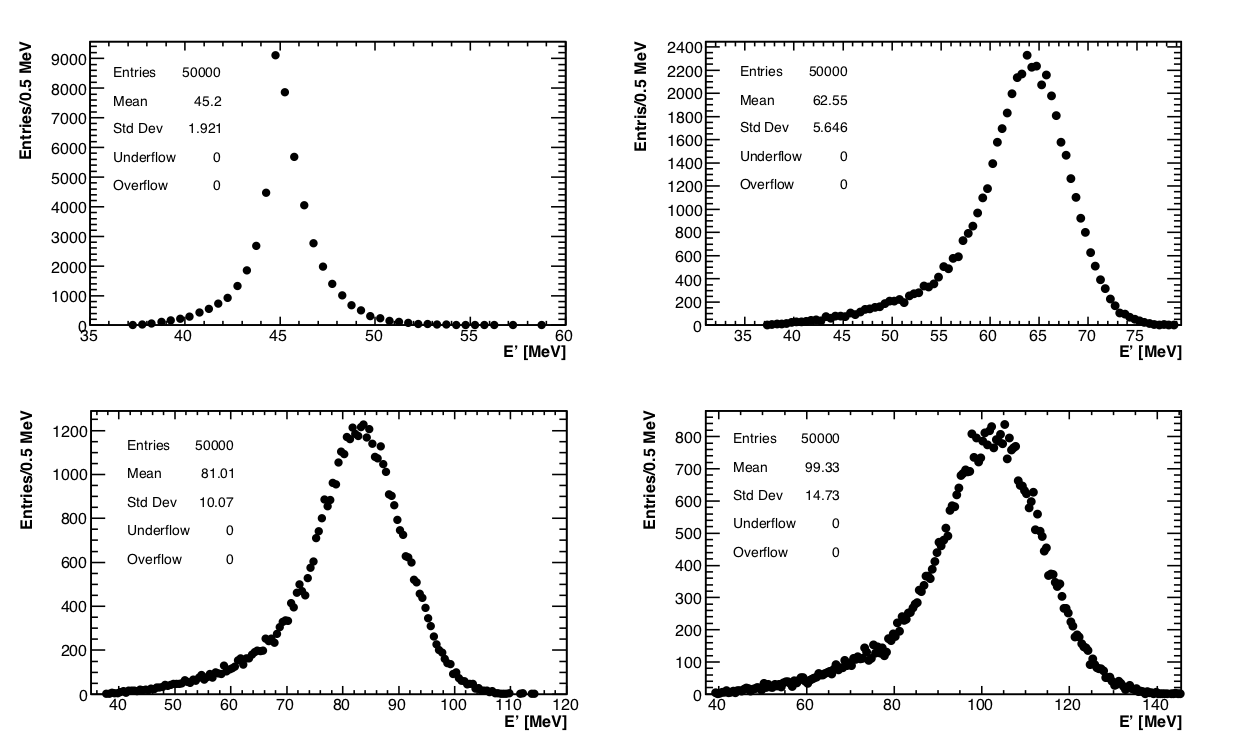
\includegraphics[width =\textwidth]{png/Resp_example98.png}
\caption{1998 detector response parametrization for different photon energies}
\label{fig:response98}
\end{figure}

In Figure~\ref{fig:shapecomp} the shape comparison of the two detector responses at 90 MeV (left) and the peaks of the detector responses as a function of the photon energies (right) are reported. The linearity of the two detector responses is similar.

\begin{figure} [!h]
\centering
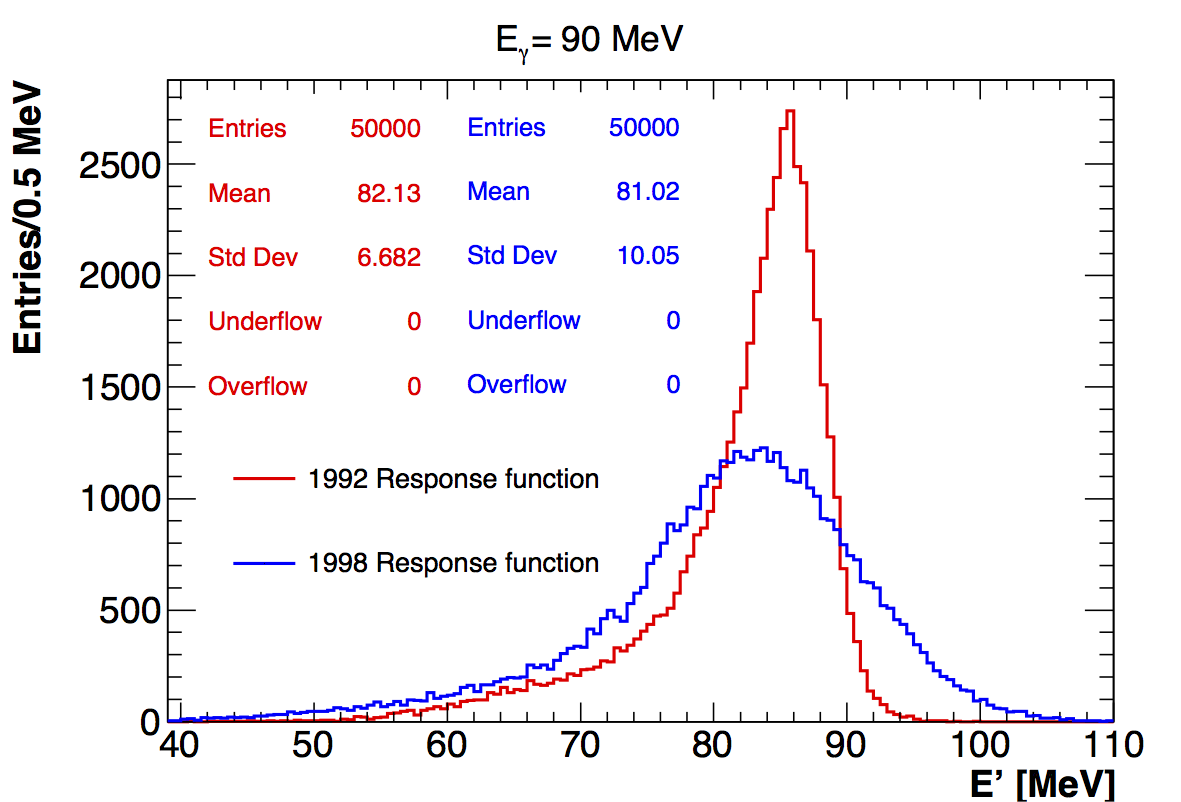
\includegraphics[width=0.49\columnwidth]{png/detRespinsieme.png}
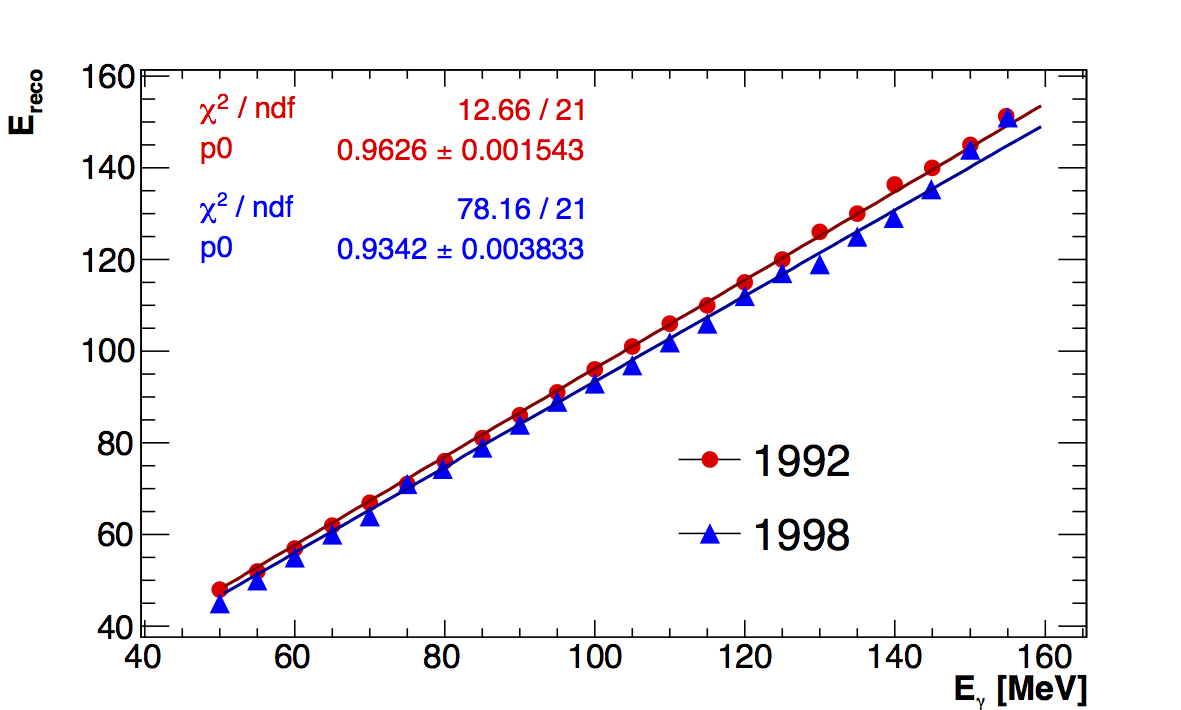
\includegraphics[width=0.49\columnwidth]{png/9298fit.png}
\caption{Left: comparison of the shape of the detector response to a 90 MeV photon. Right:peak of the detector response as a fuction of the photon energies }
\label{fig:shapecomp} 
\end{figure}

We check how well different parameterizations of the detector response describe the 
calibration peak at 129.4 MeV obtained from $\pi^{-}p \rightarrow \gamma n$ on LH$_{2}$ reported in the 1992 article.
A good agreement is shown in Figure~\ref{p004}(left) between data and  1992 response function, while the 1998 article has a completely different behaviour.\\

\begin{figure}[!h]
 \begin{center}
 \includegraphics[width=0.49\columnwidth]{png/RPC_Data_vs_1992_Response.png} 
 \includegraphics[width=0.49\columnwidth]{png/RPC_Data_vs_1998_Response.png} 
 \end{center}
 \caption{Response function of the 1992 article (left) and 1998 article (right) compared with the 129.4 MeV line from RPC on LH$_{2}$}
 \label{p004}
 \end{figure}

 In the 1998 article  however to validate  the detector response, the Radiative Pion Capture on $^{12}$Ca  is compared with the simulated data and a good agreement is reported, as shown in Figure~\ref{fig:art9}.

\begin{figure}[!h]
 \begin{center}
 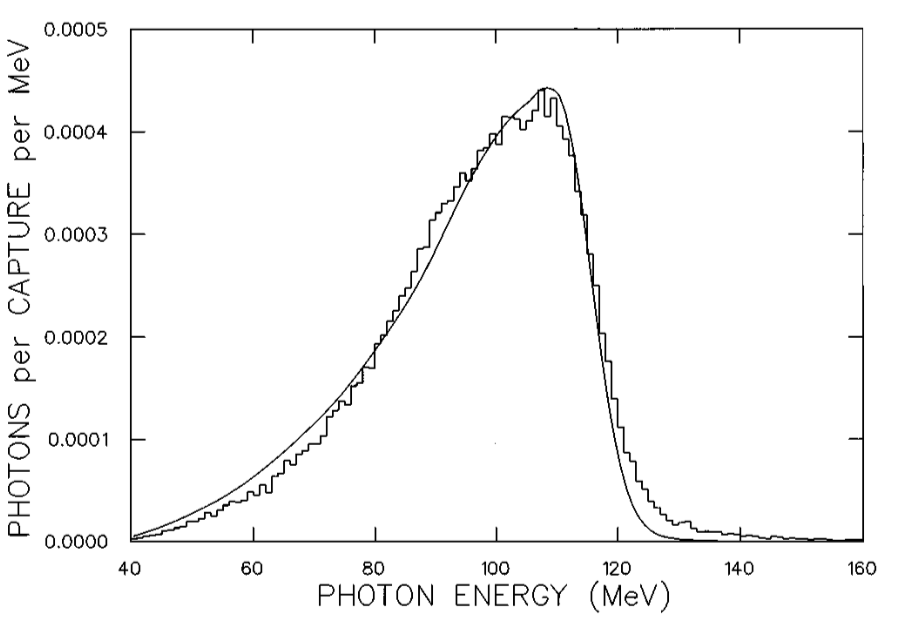
\includegraphics[width=0.45\textwidth]{png/RPC12Ca.png} 
 \end{center}
 \caption{RPC spectrum from  $\pi^{-}p \rightarrow \gamma n$ on  $^{12}$Ca compared to the simulated data }
 \label{fig:art9}
 \end{figure}
